\section{Swaption Pricing} \label{swaption_price_sec}
Now we hav seen that the implied volatility can change over various tenors. 
Therefore it is important to be aware of how the volatility affect the market.
And thereby which asset there maybe will perform in different situations i the market,
due to high or low volatility, inflation and other factor the can influence the market.
When it comes to swaption and other asset the volatility also has
a remarkable determination of the price of the asset. 
\\\\
In the Section \ref{invest_sabr} we learned how the different parameters in the 
SABR model affects the implied volatility in swaption. 
Where in Section \ref{est_parm_sabr} we estimated the parameters in the SABR model. 
From these section we saw some clear coincidence between the level of a given parameter
and the effect on the implied volatility. 
This implied volatility determine from the SABR model, is then used to price swaption using the 
Black Scholes model. 
Therefor we have computed the prices for swaption with a fixed expiry at 10 years and for various tenors. 
The price are ATM, which means that, F, the forward rate is equal to, K, 
the strike (the rate of the underlying asset). 
\\\\
Below in \autoref{tab:swaption_price_atm} the calculated prices for the various swaption 
using the describe method is listed. 
The prices are ATM prices for a fixed tenor at 10 yeas and for various tenors. 
To illustrated the development of the price over the different tenors, 
the swaption price is despited below in  \autoref{fig:swaption_price_atm}.
\\
\begin{table}[H]
  \centering
  \begin{tabular}{ccccccccccc}
    \toprule
    \textbf{ Tenor} & 1Y & 2Y & 3Y & 5Y & 7Y & 10Y & 12Y & 15Y & 20Y & 30Y \\
    \midrule
    \textbf{ Swaption price }&0.1334 & 0.1351 & 0.1360 &0.1358  &0.1336  &0.1289
    &0.1254& 0.1205 & 0.1143 & 0.1062 \\
    \bottomrule
  \end{tabular}
  \caption{ATM swaption price in basis point for a 10 years fixed expiry and various tenors.
  Data source  \\ Citi Velocity 21.02.2024}
  \label{tab:swaption_price_atm}
\end{table}

\begin{figure}[H]
    \centering
    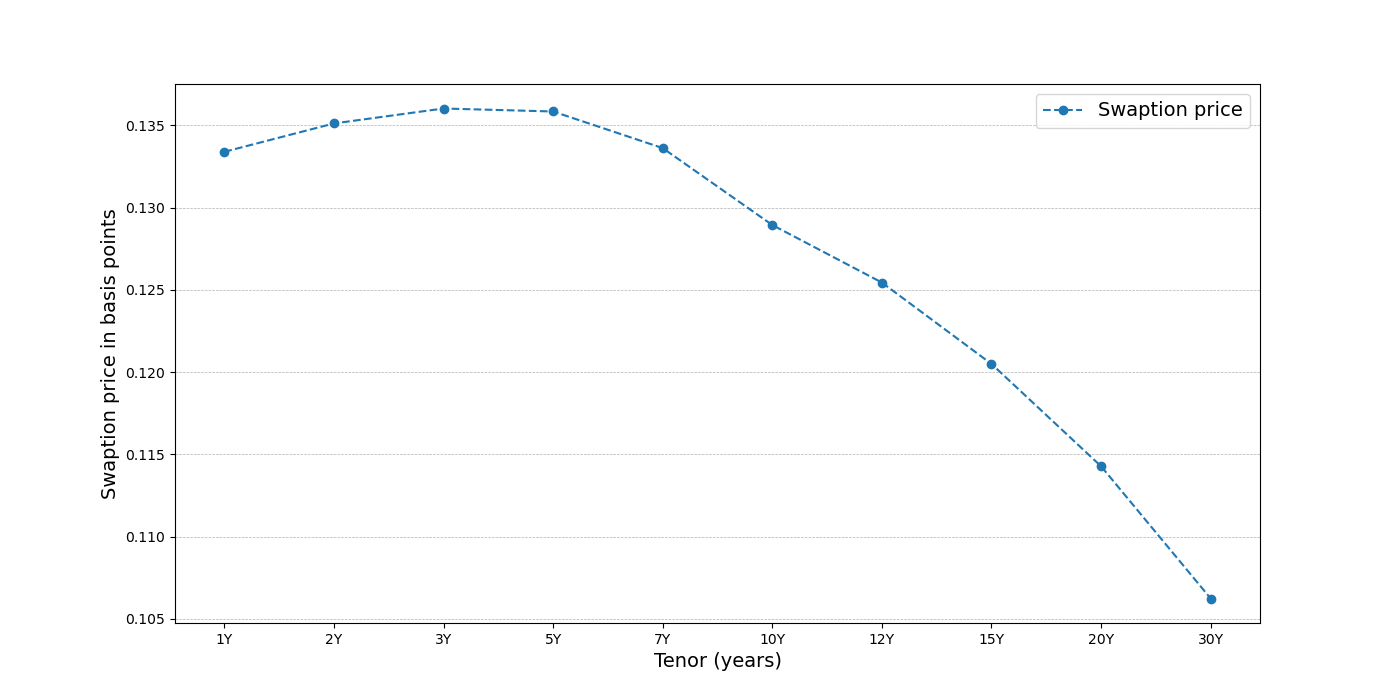
\includegraphics[width=1.\textwidth]{/Users/nannaingemannohrt/Desktop/master_thesis/main/plots/swaption_price_atm.png}
    \caption{ATM swaption price in basis point for a 10 years fixed expiry and various tenors.
    Data source  \\ Citi Velocity 21.02.2024}
    \label{fig:swaption_price_atm}
\end{figure}
\noindent